
\subsection{Bayesian Networks}
\label{subsec:int_BN}

The Bayesian Networks (also referred to as Belief Networks, Probabilistic networks or causal networks) consist of an \ac{DAG} to represent a set of conditional dependencies between random variables, that provide a compact description that allows to calculate a joint probability distribution, having in mind those dependencies into account. 

The term "Bayesian Network" were first mentioned in the literature by Judea Pearl\cite{Pearl1985}. However the idea of using networks to represent conditional relationships between variables dates to the early $20^{th}$ century with Wigmore in form of charts to analyse trial evidence\cite{Kadane1996}. 

The Figure \ref{fig:inference_relationships} provides a classical example used to understand Bayesian Networks. This example is called the ``burglary network" and it is due to Judea Pearl\cite{Pearl1988}\cite{Norvig2003}. It states a case where a person is abroad and his neighbours promise to call if they hear the alarm ring. The alarm firing is correlated with the house being robbed and the possibility of an earthquake (this example is set in Los Angeles). 

\begin{figure}[h]
\centering 

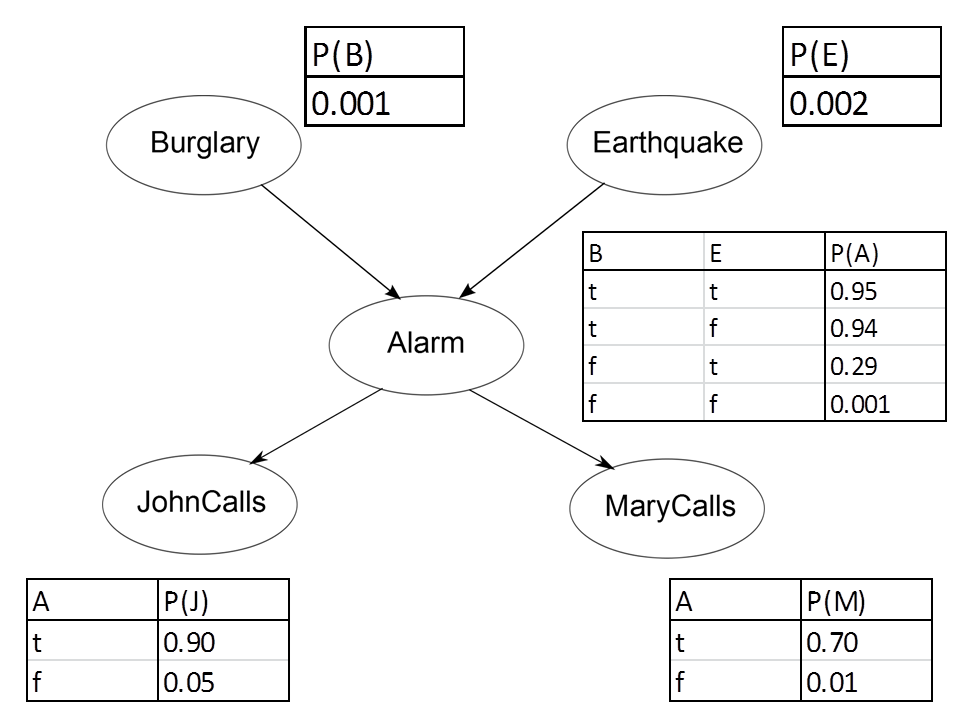
\includegraphics[scale=0.35]{Overview/Figures/BayesianNetworkExample.png}
\caption[Caption for LOF]{Burglary Network. }
\label{fig:inference_relationships}
\end{figure}
%\footnotetext{Source: \cite[Norvig and Russel 2003]{Norvig2003}}

Each node in a classical Bayesian Network represents a variable. In the example Burglary (B), Earthquake (E), Alarm (A), JohnCalls (J), and MaryCalls (M) are our random variables.
The edges represent relationships of dependency. These relationships provide elementary inference types that we can identify in the example of Figure \ref{fig:inference_relationships}. 
\begin{itemize}
\item Causation relation - A burglar(B), entering in the house makes the alarm (A), firing more likely (that's the purpose of alarms after all);
\item Diagnostic relation - The fact that the neighbours John (J) or Mary (M) call can be seen as an evidence for the alarm (A), have fired;
\item Intercausal relation - Either a burglary (B), or a earthquake (E), can cause the alarm to fire (A).
\end{itemize}

A node in a Bayesian Networks also sports a conditional probability function (represented by a \ac{CPT}). These functions consider the antecessors of the node. So for a node $X_{i}$, this would mean having access to the probability function 

\begin{equation}
\label{eq:cpt_bn}
P(X_{i} \vert Parents(X_{i} ))
\end{equation}

\ac{CPT}s for the variables considered in the previous equation. We can see that the Alarm has two antecessors (Burglary and Earthquake), so the \ac{CPT} $P(A)$, considers $P(B)$ and $P(E)$:  $P(A \vert B, E)$ as in the Equation \eqref{eq:cpt_bn}. 

The structure of the Bayesian Network allows subsets of the variables to be independent. Earthquakes don't make burglaries more likely (in the example), and Burglaries aren't known for causing earthquakes. 
Components in the networks can interact directly within a subset, despite the whole the local structure, makes this representation compact and locally structured. The set of nodes that shield a node from the rest of the network is called Markov blanket\cite{Pearl1988}. In a Bayesian Network the Markov blanket includes the parents of a node, its descendants and the parents of all its descendants. In the burglary network MaryCalls is independent of the Earthquake or the Burglary given the value of the Alarm. 

The complexity for a complete network where each variable $n$ has no more than $k$ parents is $\mathcal{O}(n.2^{k})$, this means that the complexity of a Bayesian Networks grows linearly with the number of variables, where the full joint probability on a domain grows exponentialy ($\mathcal{O}(2^{n})$). Also it is considered \cite{Pearl1985} \cite{Norvig2003} that specifying probabilities for a full joint probability table does not tally with the way human knowledge is constructed.

This makes Bayesian Networks relevant when there is a need to account for correlations between small sets of variables in a domain, providing a balance between the complexity that arises from the full joint probability table on de domain (that has the problem of exponential escalation with the increasing number of variables), and the need for models powerful enough to represent multiple dependencies. 

\subsubsection{Exact Inference}

Inference in a Bayesian Networks consists in the determination of the probability of each state in each node when there's some evidence presented.
The problem of inference in Bayesian Networks is generally NP, this made the search for optimizations and aproximations imperative. 

Considering $h$ our hypothesis variable, $e$ stands for our evidence and $Y$ are the non-evidence variables (also known as hidden or unobservable variables), we can calculate the posterior probability by enumeration, summing the terms of the full joint distribution.

\begin{equation}
P(h\vert e)=\alpha\sum_{Y}P(h,e,Y)
\end{equation}

While calculating $P(h\vert e)$ there's often repetition of calculations that cancel out. Considering an example from the burglary network, let's assume that we want to know the probability of a Burglary if both Mary and John call. This would be represented by the equation:

\begin{equation}
P(B\vert j,m)=\alpha\sum_{E}\sum_{A}P(B,j,m,A,E)
\end{equation}

By decomposing $P(B,j,m,A,E)$ using the chain rule:
\begin{equation}
P(B\vert j,m)=\alpha\sum_{E}\sum_{A}P(B).P(E).P(A\vert B,E)P(j\vert A).P(m\vert A)
\end{equation}

\begin{equation}
P(B\vert j,m)=\alpha P(B)\sum_{E}P(E)\sum_{A}P(A\vert B,E)P(j\vert A).P(m\vert A)
\end{equation}
  %imagem aqui
While computing this expression it can be seen that there are repeated sub-expressions that cancel out. In the example the following values are computed two times: 
\begin{equation}
P(j\vert A)P(m\vert A)\end{equation} and \begin{equation}P(j\vert \lnot A)P(m\vert \lnot A)\end{equation} 
Using dynamic programing can to improve the computation in the previous sittuation.

Pruning Irrelevant Variables is another way to speed up the calculation. It is considered that variables that do not belong to the evidence or the hypothesis are irrelevant unless they belong to the set comprising the ancestors of the evidence or of the hypothesis:

\begin{equation}
\label{eq:irrelevance}
Y\in\{Ancestors(\{h\}\cup e)\}
\end{equation}
In the example $P(B\vert j,m)$ $Ancestors( {B}, J, M ) = \{ A, E\}$, so there aren't irrelevant variables.
But if we take another example $P(E\vert j)$, the variable MaryCalls is irrelevant because $M \notin Antecessors( \{E\}, J ) = \{ A, B\}$.

\subsubsection{Aproximate Inference}

Given the complexity associated with exact inference, one way to fill in the \ac{CPT} of a Bayesian Network is to use approximations, namely techniques that rely on randomness. Two of this approximations techniques are:
\begin{itemize}
\item Direct Sampling Methods
\item Markov Chain Sampling
\end{itemize}

Direct sampling methods consist in using samples aquired in a training set or generated from a known probability distribution that we believe to model approximately the behaviour of the hidden variables in the network. The samples generated are used to update the \ac{CPT} of the variables in the network.

The Markov Chain Sampling assumes that the network is a system while generating samples, and it will try to make a stochastic change based on the last sample generated without disturbing evidence variables.

\subsubsection{Representing Continuous Variables}
Although the Burglary Network only has discrete stochastic variables, sometimes it's necessary to represent continuous variables.

\begin{figure}[h]
\centering 

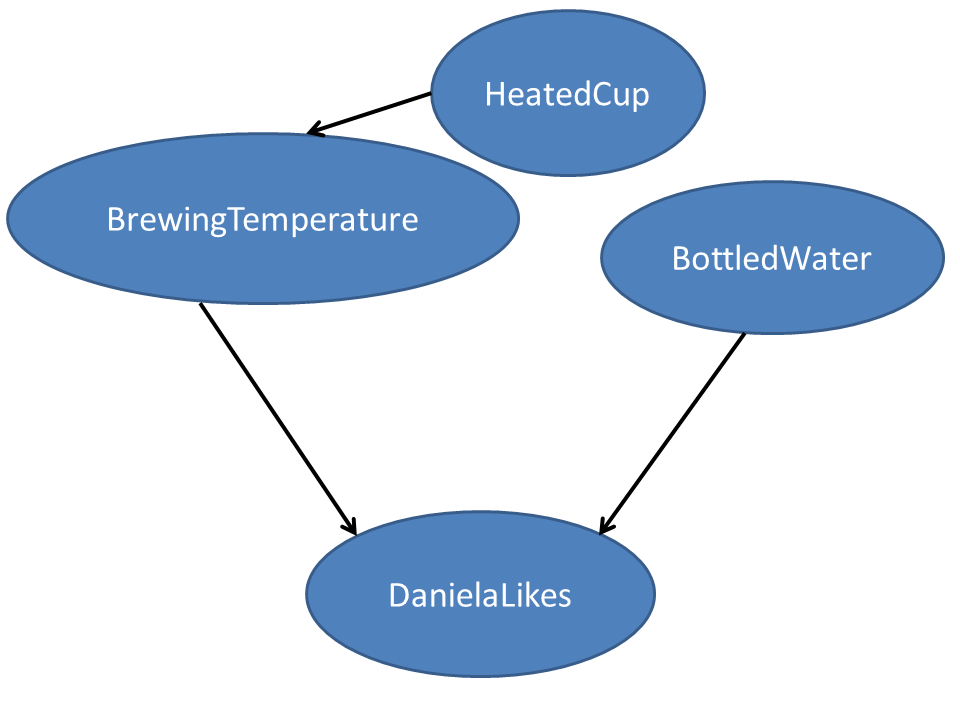
\includegraphics[scale=0.35]{Overview/Figures/TeaPreparationNetwork.png}
\caption{Tea preparation network.}
\label{fig:tea_network}
\end{figure}

One way of doing so is to create discrete intrevals, for example for the variable BrewingTemperature (representing the temperature at the end of the brewing process), in the Tea Preparation Network (Figure \ref{fig:tea_network} ), could be split in intrevals such as $T(80 > x< 85)$, but by doing so there's information that is lost.  
Other way to deal with continuous variables is to use known probabilily distributions such as the Gaussian distribution and using its parameters to model the variable. 
In the Tea preparation network where the liking of the tea is conditioned by the brewing temperature, and the brewing temperature is influenced by whether the cup was heated of not, the brewing temperature can be modeled by a Gaussian distribution. As the water is heated to a certain temperature (the mean of the distribution), the heated cup will influence directly the variations in temperature during the brewing (the more uniform the temperature during the brewing, the better), thus the standard deviation of the distribution of the Brewing temperature is conditioned by the heating of the cup.
The subject that tastes the tea will be conditioned by the use or not of bottled water and the brewing temperature. Her response to the brewing temperature can be modelled with a sigmoid function to reflect the liking or not.
A Bayesian Network with both discrete and continuous variables is called an hybrid network.


\subsubsection{Dynamic Bayesian Networks}
\ac{DBN}, also known as Two-Timeslice Bayesian Networks, are an extension of the common Bayesian Network to deal with a temporal evolution\cite{eemcs5901}. \ac{DBN} have resemblances to \ac{HMM}. More accurately we can say that \ac{HMM} are special cases of \ac{DBN}, a \ac{DBN} single discrete state variable\cite{Norvig2003}. 

The temporal dimension in \ac{DBN} is represented as time-steps. Each time step corresponds to a classical Bayesian Network, but the nodes in this Bayesian Network can have temporal links, represented as a directed edge to the next time-step, this means that these nodes will have influence on the variables of the nodes they connect with, in the following time-step.

\begin{figure}[h]
\centering 

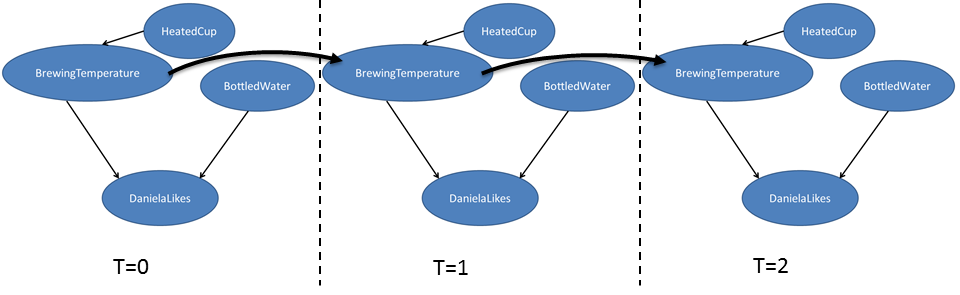
\includegraphics[scale=0.48]{Overview/Figures/TeaPreparationNetworkDBN.png}
\caption{Time evolution of the ``Tea preparation network".}
\label{fig:tea_networkdbn}
\end{figure}

In the Figure \ref{fig:tea_networkdbn} we have a possible transformation of the example of the ``Tea Preparation" to accommodate a time evolution. The variable Brewing Temperature at a given time-step will depend on the brewing temperature in the previous measurement (empiricaly we know that the temperature will not increase given the last time-step). 



\begin{comment}
Unlike the other two sampling algorithms, which generate each event from scratch, MCMC generates each event by making a random change to the preceding event. It is therefore helpful to think of the network as being in a particular current state specifying a value for every variable. The next state is generated by randomly sampling a value for one of the non-evidence variables Xi,
conditioned on the current values of the variables in the Markov
blanket of Xi. (Recall

 and requires a large amount of statistical data to 
his suggests that the elementary building blocks which make up human knowledge are not the entries of a joint-distribution table, but rather the low-order marginal and conditional probabilities defined over small clusters of propositions.


\end{comment}


%Examples???